\section{Première formulation robuste}
\subsection{Modèle}
Afin de prendre en compte les erreurs sur les facteurs d'amplification $x_i$, nous utilisons les valeurs maximales des variations possibles de $\hat{D(\theta)}$ sur un intervalle.\\
\begin{eqnarray}
|\hat{D(\theta)}| & = & |\sum_{i=1}^{n} x_i(1+\xi_i)d_i(\theta)| \nonumber \\
& \leq & |\sum_{i=1}^{n} x_i d_i(\theta)| + |\sum_{i=1}^{n} x_i \xi_i d_i(\theta)| \nonumber \\
& \leq & |D(\theta)| + \sum_{i=1}^{n} |\tau d_i(\theta)\frac{h}{2}| \nonumber
\end{eqnarray}
En imposant 
$$|D(\theta)| + \sum_{i=1}^{n} |\tau d_i(\theta)\frac{h}{2}|\leq \epsilon $$
on est sur que $|\hat{D(\theta)}|\leq \epsilon$. De la même manière, on traduit les contraintes sur P : 
$$|D(\theta)-1| + \sum_{i=1}^{n} |\tau d_i(\theta)\frac{h}{2}|\leq \epsilon $$
Il nous faut donc introduire n variables $v_i$ pour chaque $\theta$ échantillonné, correspondant aux valeurs absolues des $\tau d_i(\theta)\frac{h}{2}$
On a alors 
\begin{eqnarray}
|D(\theta)| + \sum_{i=1}^{n} |\tau x_i d_i(\theta)\frac{h}{2}| & \leq & \epsilon \nonumber \\
|D(\theta)-1| + \sum_{i=1}^{n} |\tau x_i d_i(\theta)\frac{h}{2}| & \leq & \epsilon \nonumber \\
\tau x_i d_i(\theta)\frac{h}{2} & \leq & v_i \nonumber \\
-\tau x_i d_i(\theta)\frac{h}{2} & \leq & v_i \nonumber 
\end{eqnarray}

\subsection{Analyse des résultats}
Les figures \ref{fig:D-ModRobust1-01}, \ref{fig:D-ModRobust1-001}, \ref{fig:D-ModRobust1-testRob01} et \ref{fig:D-ModRobust1-testRob001} montrent les résultats obtenus pour différentes valeurs de $\tau$. Ici les $x$ sont conçus pour mieux résister en cas de perturbations. \\
Dans le cas $\tau = 0.01$, on souhaite que les $x$ résiste à de plus grande perturbation, ainsi le $\epsilon$ est plus grand ($3.3 \%$) mais les perturbations sont moins dommageables (oscillations moins grandes sur la figure \ref{fig:D-ModRobust1-testRob01} que sur \ref{fig:D-ModRobust1-testRob001}).\\
Dans le cas $\tau = 0.01$, on souhaite que les $x$ résiste à de plus petites perturbation, ainsi le $\epsilon$ est moins grand ($2.8 \%$) mais les perturbations sont plus dommageables.\\
Notons que ce modèle est bien plus performant que le mode de base. En effet le $\epsilon$ augmente très peu $2\%$ dans le modèle de base à $2.8\%$ ou $3.3\%$ dans le modèle robuste; tandis que la robustesse s'améliore nettement.

\begin{figure}[h!]
  \centering
  \begin{subfigure}[b]{0.45\textwidth}
  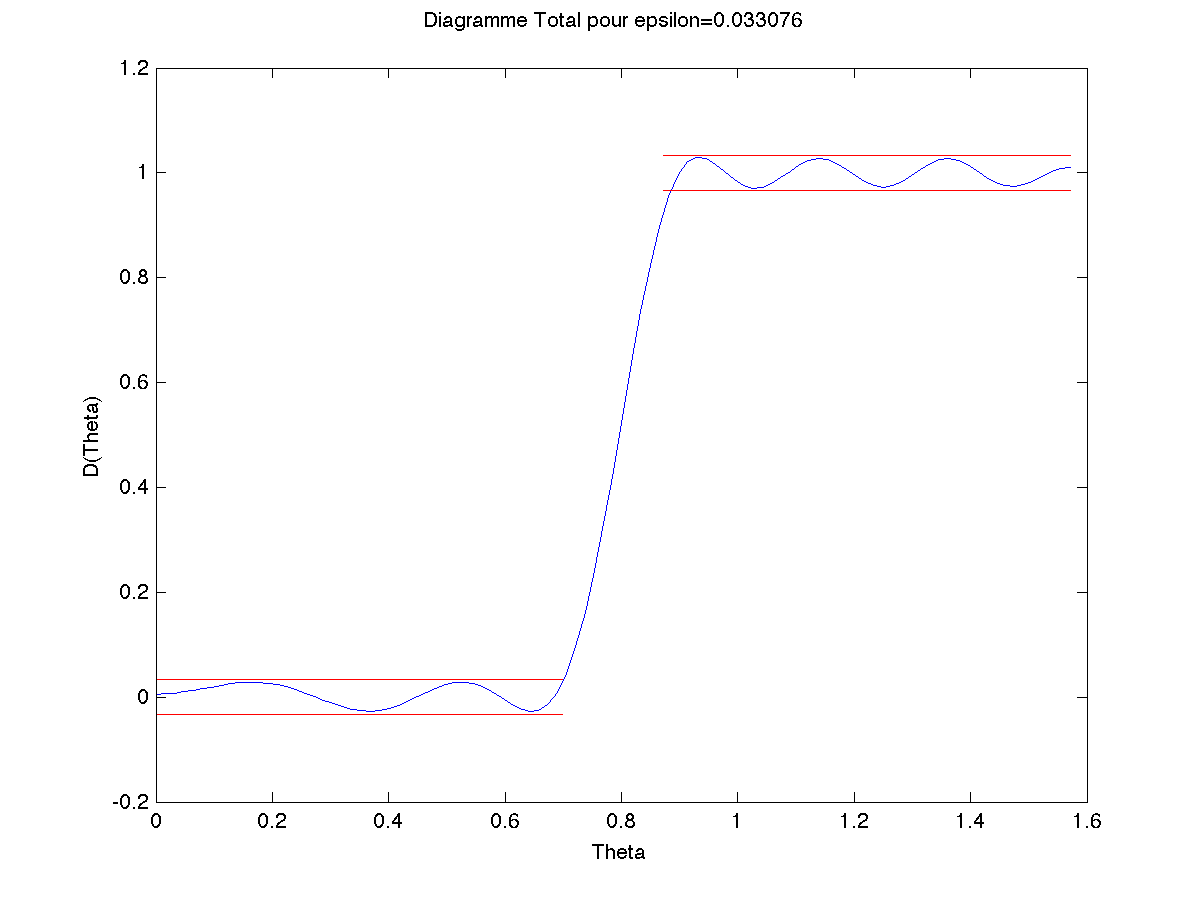
\includegraphics[width=\textwidth]{D-ModRobust1-01.png}
  \caption{$D(\theta)$ pour $\tau = 0.01$ et $x$ non-perturbé.}
  \label{fig:D-ModRobust1-01}
  \end{subfigure}%
  ~ 
  \begin{subfigure}[b]{0.45\textwidth}
  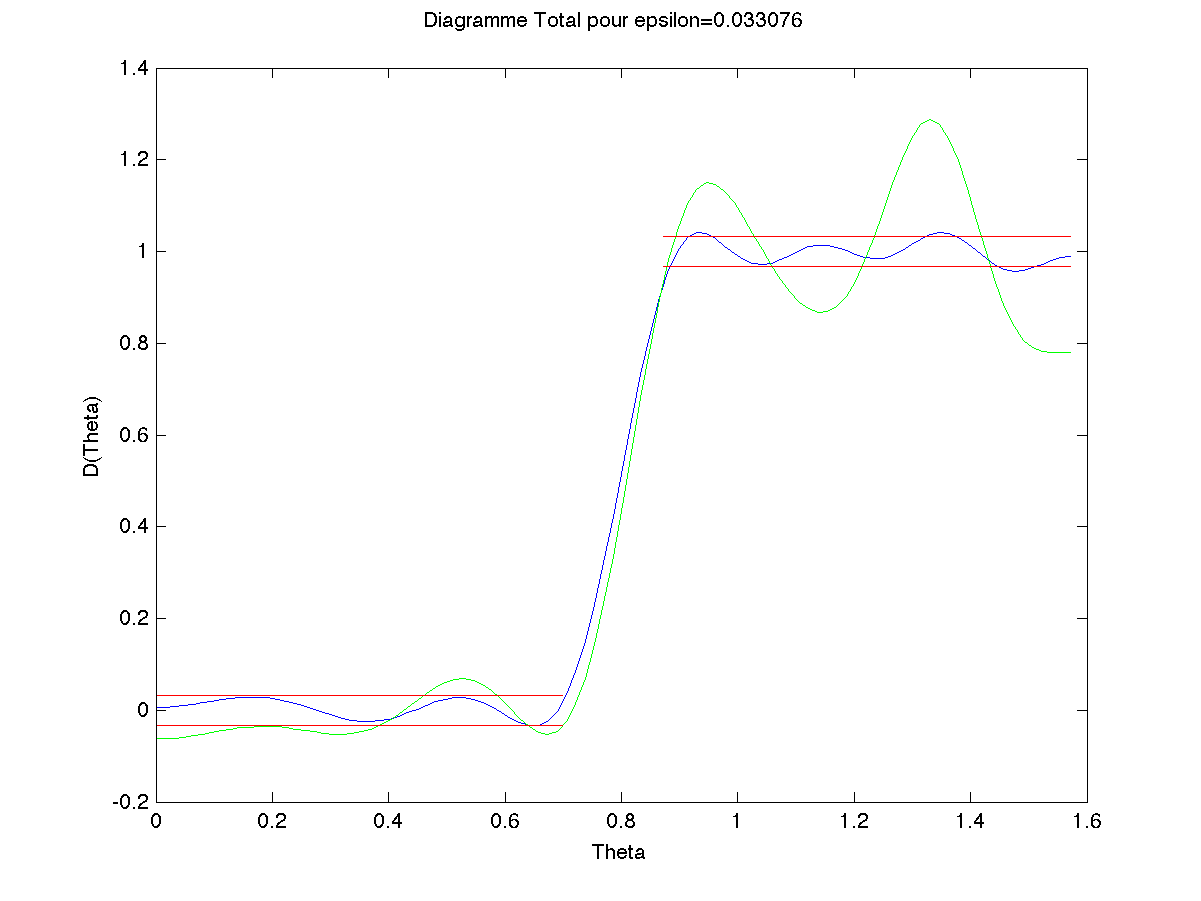
\includegraphics[width=\textwidth]{D-ModRobust1-testRob01.png}
  \caption{$D(\theta)$ pour $\tau = 0.01$ et $x$ perturbés (en vert pour une perturbation de $\tau=0.01$ en bleu pour $\tau=0.001$).}
  \label{fig:D-ModRobust1-testRob01}
  \end{subfigure}
  \begin{subfigure}[b]{0.45\textwidth}
  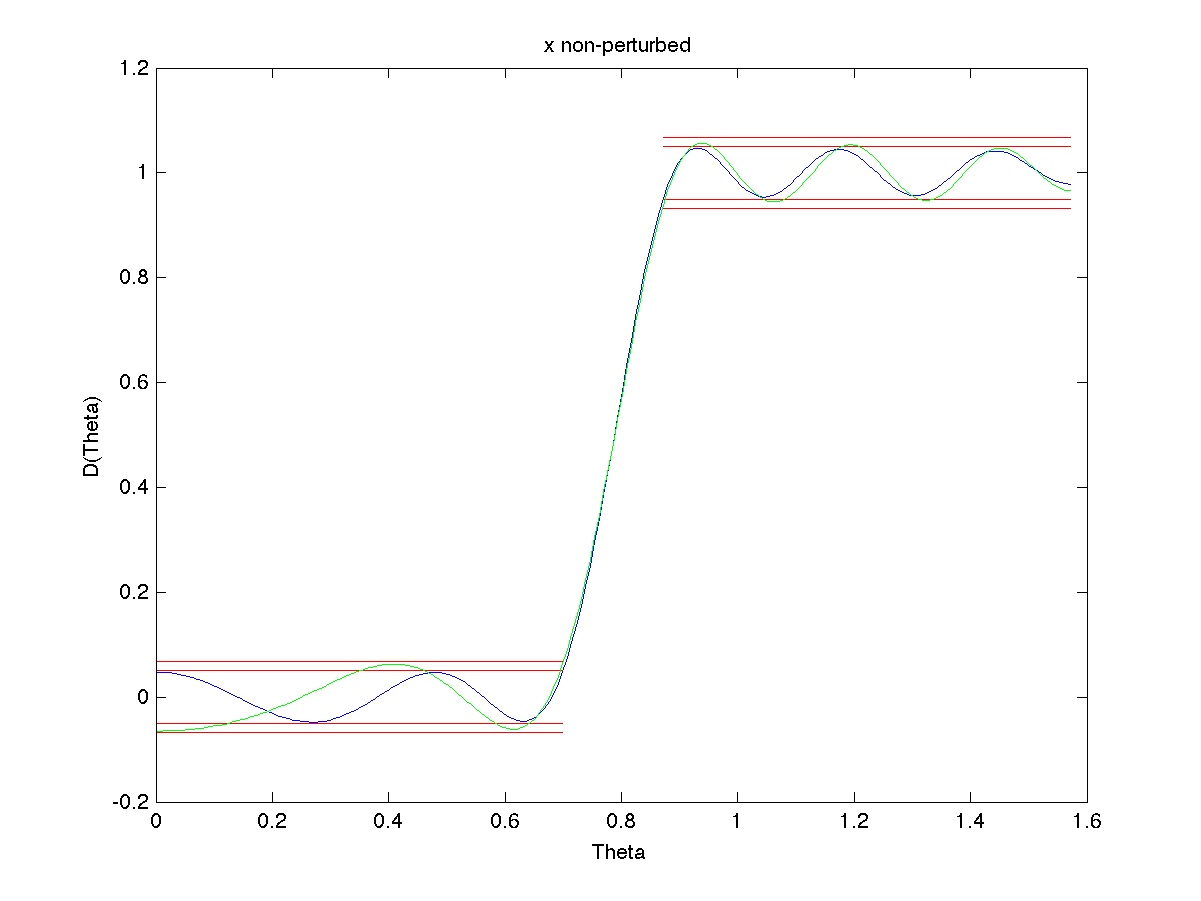
\includegraphics[width=\textwidth]{D-ModRobust1-001.png}
  \caption{$D(\theta)$ pour $\tau = 0.001$ et $x$ non-perturbé.}
  \label{fig:D-ModRobust1-001}
  \end{subfigure}%
  ~ 
  \begin{subfigure}[b]{0.45\textwidth}
  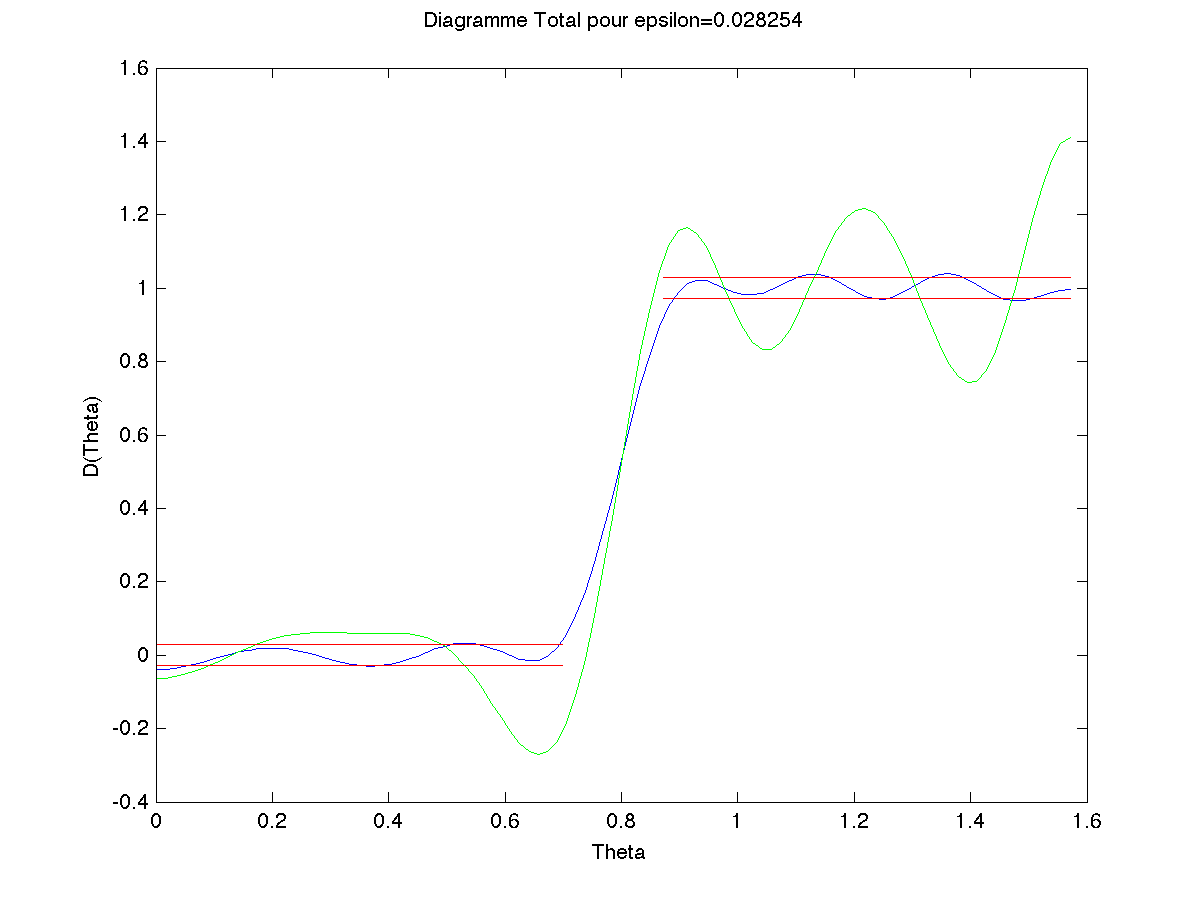
\includegraphics[width=\textwidth]{D-ModRobust1-testRob001.png}
  \caption{$D(\theta)$ pour $\tau = 0.001$ et $x$ perturbés (en vert pour une perturbation de $\tau=0.01$ en bleu pour $\tau=0.001$).}
  \label{fig:D-ModRobust1-testRob001}
  \end{subfigure}
  \caption{}
  \end{figure}
